% Created by tikzDevice version 0.6.2-92-0ad2792 on 2013-03-12 18:53:48
% !TEX encoding = UTF-8 Unicode
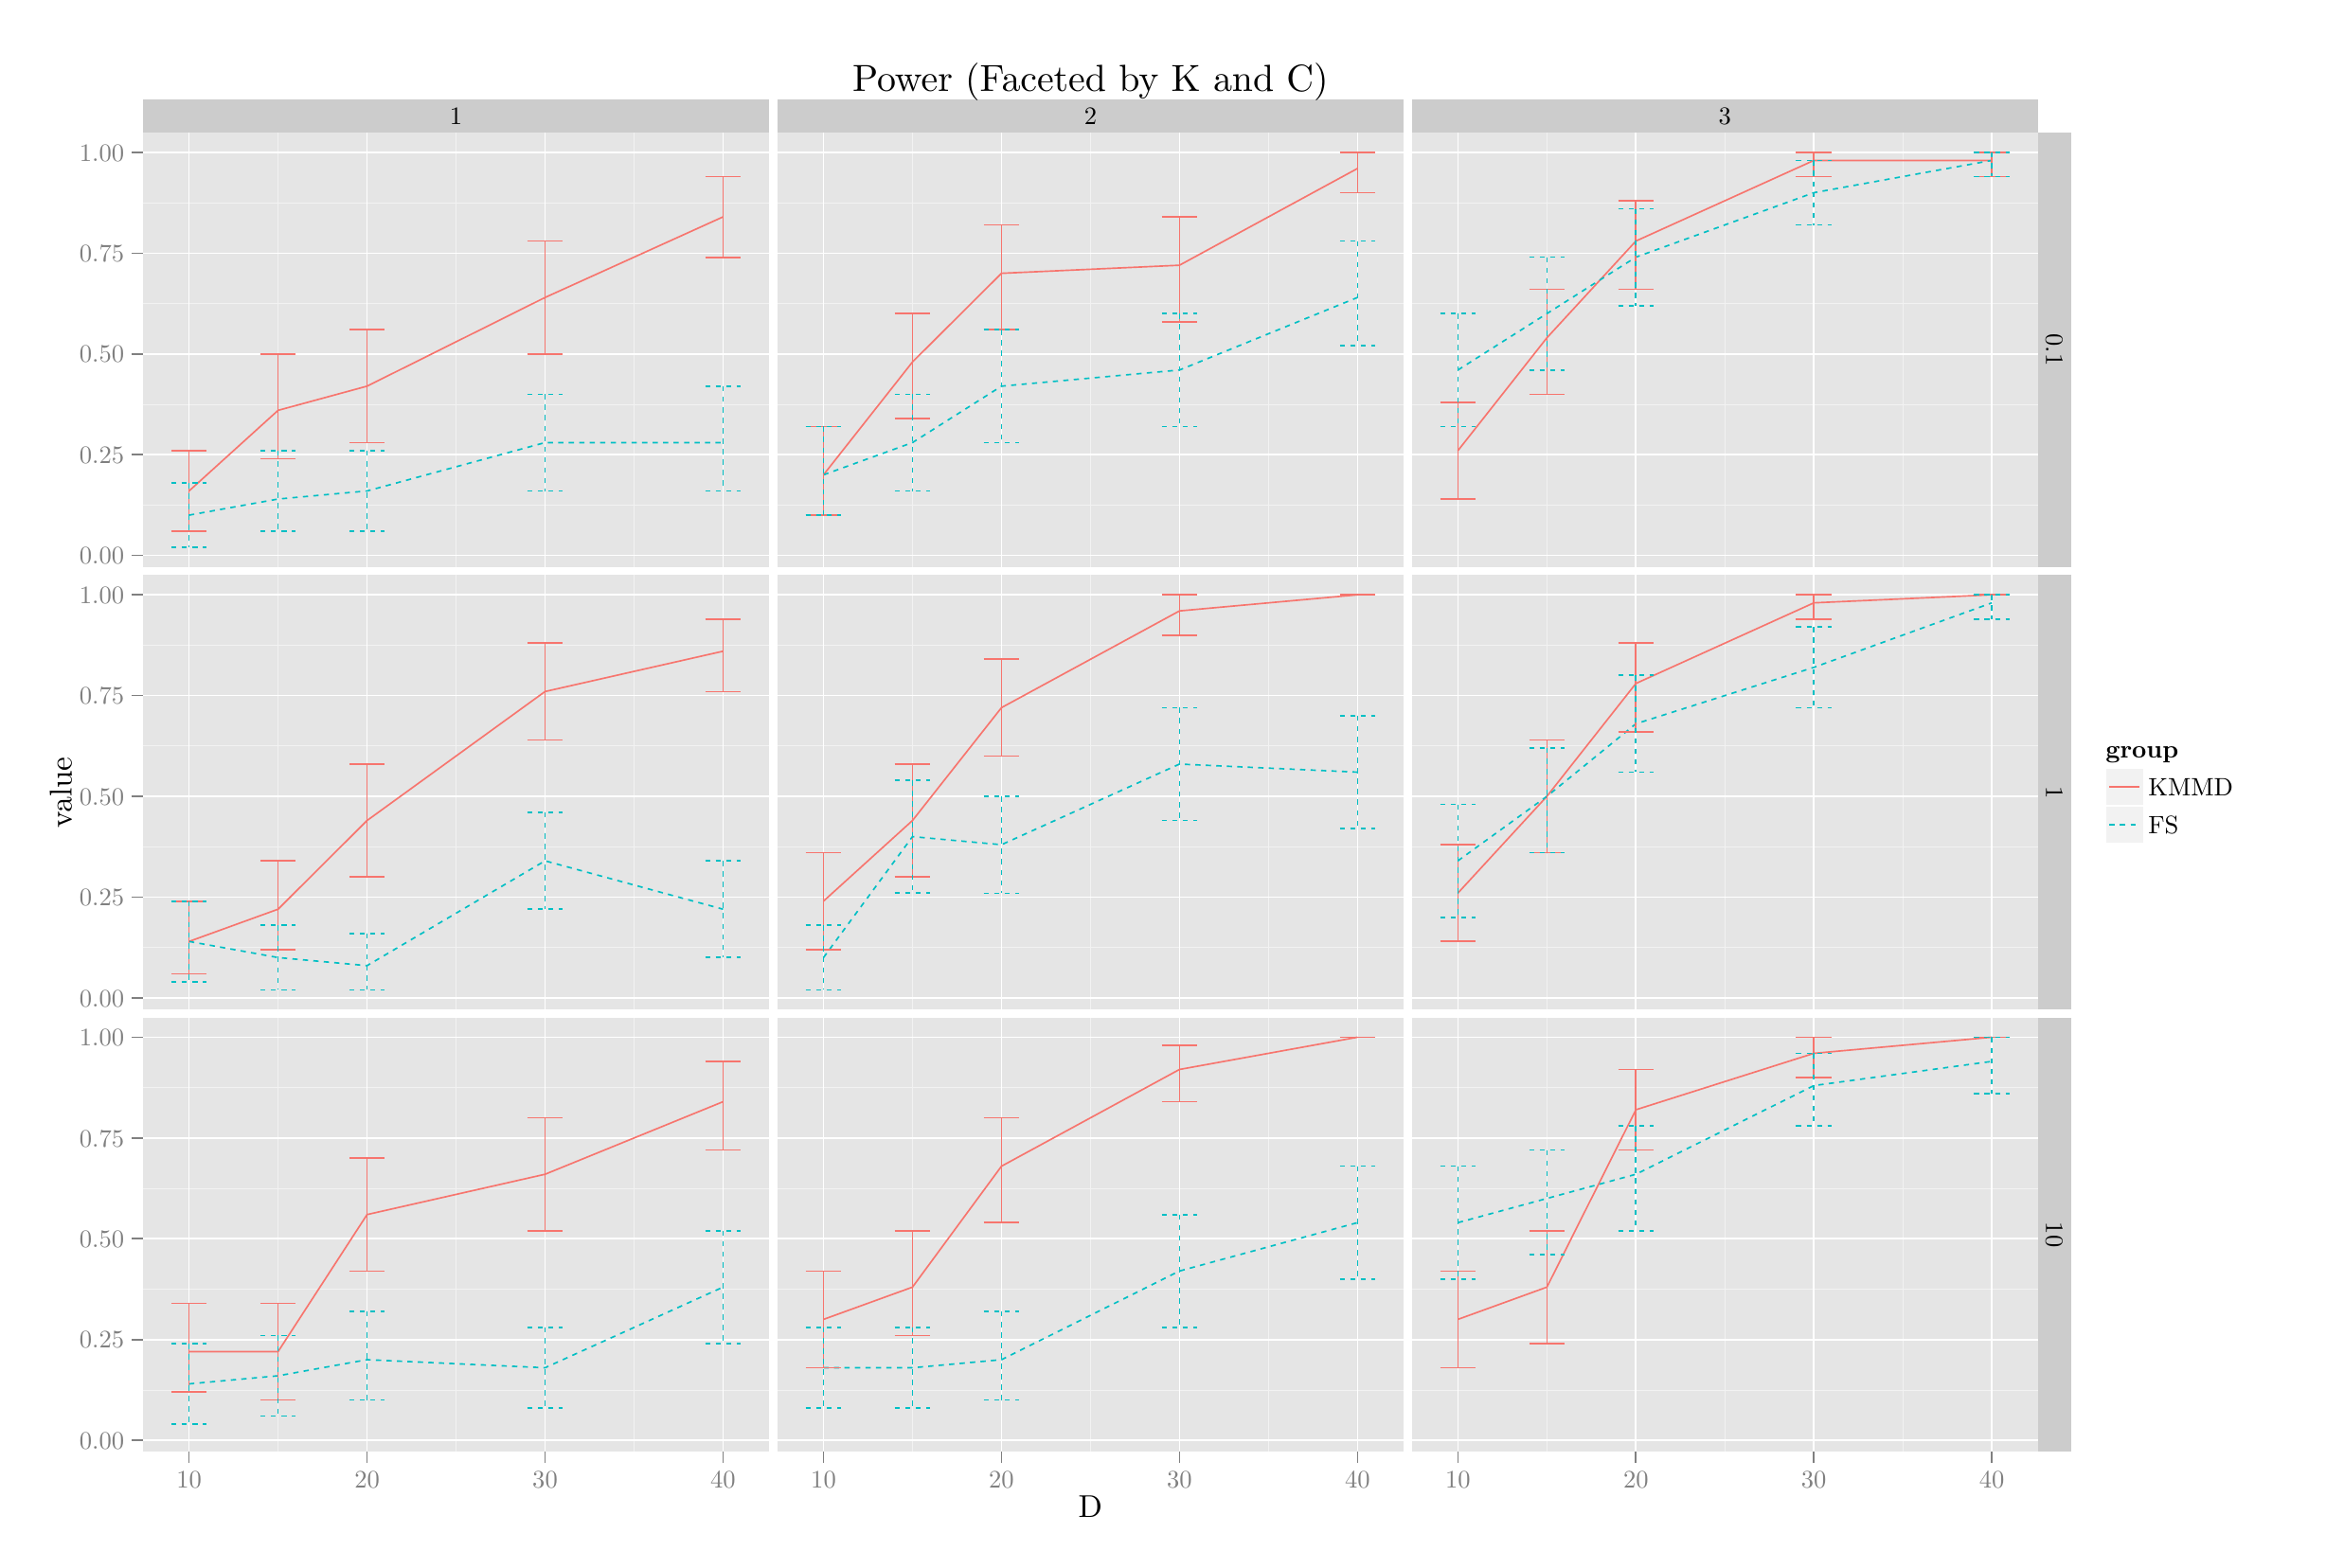
\begin{tikzpicture}[x=1pt,y=1pt]
\definecolor[named]{fillColor}{rgb}{1.00,1.00,1.00}
\path[use as bounding box,fill=fillColor,fill opacity=0.00] (0,0) rectangle (867.24,578.16);
\begin{scope}
\path[clip] (  0.00,  0.00) rectangle (867.24,578.16);
\definecolor[named]{drawColor}{rgb}{1.00,1.00,1.00}
\definecolor[named]{fillColor}{rgb}{1.00,1.00,1.00}

\path[draw=drawColor,line width= 0.6pt,line join=round,line cap=round,fill=fillColor] (  0.00, -0.00) rectangle (867.24,578.16);
\end{scope}
\begin{scope}
\path[clip] ( 44.49,537.54) rectangle (283.53,550.17);
\definecolor[named]{fillColor}{rgb}{0.80,0.80,0.80}

\path[fill=fillColor] ( 44.49,537.54) rectangle (283.53,550.17);
\definecolor[named]{drawColor}{rgb}{0.00,0.00,0.00}

\node[text=drawColor,anchor=base,inner sep=0pt, outer sep=0pt, scale=  0.96] at (164.01,540.55) {1};
\end{scope}
\begin{scope}
\path[clip] (286.54,537.54) rectangle (525.58,550.17);
\definecolor[named]{fillColor}{rgb}{0.80,0.80,0.80}

\path[fill=fillColor] (286.54,537.54) rectangle (525.58,550.17);
\definecolor[named]{drawColor}{rgb}{0.00,0.00,0.00}

\node[text=drawColor,anchor=base,inner sep=0pt, outer sep=0pt, scale=  0.96] at (406.06,540.55) {2};
\end{scope}
\begin{scope}
\path[clip] (528.59,537.54) rectangle (767.64,550.17);
\definecolor[named]{fillColor}{rgb}{0.80,0.80,0.80}

\path[fill=fillColor] (528.59,537.54) rectangle (767.64,550.17);
\definecolor[named]{drawColor}{rgb}{0.00,0.00,0.00}

\node[text=drawColor,anchor=base,inner sep=0pt, outer sep=0pt, scale=  0.96] at (648.11,540.55) {3};
\end{scope}
\begin{scope}
\path[clip] ( 44.49,371.71) rectangle (283.53,537.54);
\definecolor[named]{fillColor}{rgb}{0.90,0.90,0.90}

\path[fill=fillColor] ( 44.49,371.71) rectangle (283.53,537.54);
\definecolor[named]{drawColor}{rgb}{0.95,0.95,0.95}

\path[draw=drawColor,line width= 0.3pt,line join=round] ( 44.49,395.40) --
	(283.53,395.40);

\path[draw=drawColor,line width= 0.3pt,line join=round] ( 44.49,433.86) --
	(283.53,433.86);

\path[draw=drawColor,line width= 0.3pt,line join=round] ( 44.49,472.32) --
	(283.53,472.32);

\path[draw=drawColor,line width= 0.3pt,line join=round] ( 44.49,510.77) --
	(283.53,510.77);

\path[draw=drawColor,line width= 0.3pt,line join=round] ( 96.10,371.71) --
	( 96.10,537.54);

\path[draw=drawColor,line width= 0.3pt,line join=round] (164.01,371.71) --
	(164.01,537.54);

\path[draw=drawColor,line width= 0.3pt,line join=round] (231.92,371.71) --
	(231.92,537.54);
\definecolor[named]{drawColor}{rgb}{1.00,1.00,1.00}

\path[draw=drawColor,line width= 0.6pt,line join=round] ( 44.49,376.17) --
	(283.53,376.17);

\path[draw=drawColor,line width= 0.6pt,line join=round] ( 44.49,414.63) --
	(283.53,414.63);

\path[draw=drawColor,line width= 0.6pt,line join=round] ( 44.49,453.09) --
	(283.53,453.09);

\path[draw=drawColor,line width= 0.6pt,line join=round] ( 44.49,491.55) --
	(283.53,491.55);

\path[draw=drawColor,line width= 0.6pt,line join=round] ( 44.49,530.00) --
	(283.53,530.00);

\path[draw=drawColor,line width= 0.6pt,line join=round] ( 62.14,371.71) --
	( 62.14,537.54);

\path[draw=drawColor,line width= 0.6pt,line join=round] (130.05,371.71) --
	(130.05,537.54);

\path[draw=drawColor,line width= 0.6pt,line join=round] (197.96,371.71) --
	(197.96,537.54);

\path[draw=drawColor,line width= 0.6pt,line join=round] (265.87,371.71) --
	(265.87,537.54);
\definecolor[named]{drawColor}{rgb}{0.97,0.46,0.43}

\path[draw=drawColor,line width= 0.6pt,line join=round] ( 62.14,400.79) --
	( 96.10,431.55) --
	(130.05,440.78) --
	(197.96,474.62) --
	(265.87,505.39);
\definecolor[named]{drawColor}{rgb}{0.00,0.75,0.77}

\path[draw=drawColor,line width= 0.6pt,dash pattern=on 2pt off 2pt ,line join=round] ( 62.14,391.56) --
	( 96.10,397.71) --
	(130.05,400.79) --
	(197.96,419.25) --
	(265.87,419.25);
\definecolor[named]{drawColor}{rgb}{0.97,0.46,0.43}

\path[draw=drawColor,line width= 0.6pt,line join=round] ( 55.35,416.25) --
	( 68.93,416.25);

\path[draw=drawColor,line width= 0.6pt,line join=round] ( 62.14,416.25) --
	( 62.14,385.40);

\path[draw=drawColor,line width= 0.6pt,line join=round] ( 55.35,385.40) --
	( 68.93,385.40);

\path[draw=drawColor,line width= 0.6pt,line join=round] ( 89.31,453.09) --
	(102.89,453.09);

\path[draw=drawColor,line width= 0.6pt,line join=round] ( 96.10,453.09) --
	( 96.10,413.09);

\path[draw=drawColor,line width= 0.6pt,line join=round] ( 89.31,413.09) --
	(102.89,413.09);

\path[draw=drawColor,line width= 0.6pt,line join=round] (123.26,462.32) --
	(136.84,462.32);

\path[draw=drawColor,line width= 0.6pt,line join=round] (130.05,462.32) --
	(130.05,419.25);

\path[draw=drawColor,line width= 0.6pt,line join=round] (123.26,419.25) --
	(136.84,419.25);

\path[draw=drawColor,line width= 0.6pt,line join=round] (191.17,496.16) --
	(204.75,496.16);

\path[draw=drawColor,line width= 0.6pt,line join=round] (197.96,496.16) --
	(197.96,453.09);

\path[draw=drawColor,line width= 0.6pt,line join=round] (191.17,453.09) --
	(204.75,453.09);

\path[draw=drawColor,line width= 0.6pt,line join=round] (259.08,520.77) --
	(272.66,520.77);

\path[draw=drawColor,line width= 0.6pt,line join=round] (265.87,520.77) --
	(265.87,489.93);

\path[draw=drawColor,line width= 0.6pt,line join=round] (259.08,489.93) --
	(272.66,489.93);
\definecolor[named]{drawColor}{rgb}{0.00,0.75,0.77}

\path[draw=drawColor,line width= 0.6pt,dash pattern=on 2pt off 2pt ,line join=round] ( 55.35,403.86) --
	( 68.93,403.86);

\path[draw=drawColor,line width= 0.6pt,dash pattern=on 2pt off 2pt ,line join=round] ( 62.14,403.86) --
	( 62.14,379.25);

\path[draw=drawColor,line width= 0.6pt,dash pattern=on 2pt off 2pt ,line join=round] ( 55.35,379.25) --
	( 68.93,379.25);

\path[draw=drawColor,line width= 0.6pt,dash pattern=on 2pt off 2pt ,line join=round] ( 89.31,416.17) --
	(102.89,416.17);

\path[draw=drawColor,line width= 0.6pt,dash pattern=on 2pt off 2pt ,line join=round] ( 96.10,416.17) --
	( 96.10,385.40);

\path[draw=drawColor,line width= 0.6pt,dash pattern=on 2pt off 2pt ,line join=round] ( 89.31,385.40) --
	(102.89,385.40);

\path[draw=drawColor,line width= 0.6pt,dash pattern=on 2pt off 2pt ,line join=round] (123.26,416.17) --
	(136.84,416.17);

\path[draw=drawColor,line width= 0.6pt,dash pattern=on 2pt off 2pt ,line join=round] (130.05,416.17) --
	(130.05,385.40);

\path[draw=drawColor,line width= 0.6pt,dash pattern=on 2pt off 2pt ,line join=round] (123.26,385.40) --
	(136.84,385.40);

\path[draw=drawColor,line width= 0.6pt,dash pattern=on 2pt off 2pt ,line join=round] (191.17,437.71) --
	(204.75,437.71);

\path[draw=drawColor,line width= 0.6pt,dash pattern=on 2pt off 2pt ,line join=round] (197.96,437.71) --
	(197.96,400.79);

\path[draw=drawColor,line width= 0.6pt,dash pattern=on 2pt off 2pt ,line join=round] (191.17,400.79) --
	(204.75,400.79);

\path[draw=drawColor,line width= 0.6pt,dash pattern=on 2pt off 2pt ,line join=round] (259.08,440.78) --
	(272.66,440.78);

\path[draw=drawColor,line width= 0.6pt,dash pattern=on 2pt off 2pt ,line join=round] (265.87,440.78) --
	(265.87,400.79);

\path[draw=drawColor,line width= 0.6pt,dash pattern=on 2pt off 2pt ,line join=round] (259.08,400.79) --
	(272.66,400.79);
\end{scope}
\begin{scope}
\path[clip] ( 44.49,202.87) rectangle (283.53,368.70);
\definecolor[named]{fillColor}{rgb}{0.90,0.90,0.90}

\path[fill=fillColor] ( 44.49,202.87) rectangle (283.53,368.70);
\definecolor[named]{drawColor}{rgb}{0.95,0.95,0.95}

\path[draw=drawColor,line width= 0.3pt,line join=round] ( 44.49,226.56) --
	(283.53,226.56);

\path[draw=drawColor,line width= 0.3pt,line join=round] ( 44.49,265.02) --
	(283.53,265.02);

\path[draw=drawColor,line width= 0.3pt,line join=round] ( 44.49,303.48) --
	(283.53,303.48);

\path[draw=drawColor,line width= 0.3pt,line join=round] ( 44.49,341.94) --
	(283.53,341.94);

\path[draw=drawColor,line width= 0.3pt,line join=round] ( 96.10,202.87) --
	( 96.10,368.70);

\path[draw=drawColor,line width= 0.3pt,line join=round] (164.01,202.87) --
	(164.01,368.70);

\path[draw=drawColor,line width= 0.3pt,line join=round] (231.92,202.87) --
	(231.92,368.70);
\definecolor[named]{drawColor}{rgb}{1.00,1.00,1.00}

\path[draw=drawColor,line width= 0.6pt,line join=round] ( 44.49,207.33) --
	(283.53,207.33);

\path[draw=drawColor,line width= 0.6pt,line join=round] ( 44.49,245.79) --
	(283.53,245.79);

\path[draw=drawColor,line width= 0.6pt,line join=round] ( 44.49,284.25) --
	(283.53,284.25);

\path[draw=drawColor,line width= 0.6pt,line join=round] ( 44.49,322.71) --
	(283.53,322.71);

\path[draw=drawColor,line width= 0.6pt,line join=round] ( 44.49,361.16) --
	(283.53,361.16);

\path[draw=drawColor,line width= 0.6pt,line join=round] ( 62.14,202.87) --
	( 62.14,368.70);

\path[draw=drawColor,line width= 0.6pt,line join=round] (130.05,202.87) --
	(130.05,368.70);

\path[draw=drawColor,line width= 0.6pt,line join=round] (197.96,202.87) --
	(197.96,368.70);

\path[draw=drawColor,line width= 0.6pt,line join=round] (265.87,202.87) --
	(265.87,368.70);
\definecolor[named]{drawColor}{rgb}{0.97,0.46,0.43}

\path[draw=drawColor,line width= 0.6pt,line join=round] ( 62.14,228.87) --
	( 96.10,241.18) --
	(130.05,275.02) --
	(197.96,324.24) --
	(265.87,339.63);
\definecolor[named]{drawColor}{rgb}{0.00,0.75,0.77}

\path[draw=drawColor,line width= 0.6pt,dash pattern=on 2pt off 2pt ,line join=round] ( 62.14,228.87) --
	( 96.10,222.72) --
	(130.05,219.64) --
	(197.96,259.64) --
	(265.87,241.18);
\definecolor[named]{drawColor}{rgb}{0.97,0.46,0.43}

\path[draw=drawColor,line width= 0.6pt,line join=round] ( 55.35,244.25) --
	( 68.93,244.25);

\path[draw=drawColor,line width= 0.6pt,line join=round] ( 62.14,244.25) --
	( 62.14,216.56);

\path[draw=drawColor,line width= 0.6pt,line join=round] ( 55.35,216.56) --
	( 68.93,216.56);

\path[draw=drawColor,line width= 0.6pt,line join=round] ( 89.31,259.64) --
	(102.89,259.64);

\path[draw=drawColor,line width= 0.6pt,line join=round] ( 96.10,259.64) --
	( 96.10,225.79);

\path[draw=drawColor,line width= 0.6pt,line join=round] ( 89.31,225.79) --
	(102.89,225.79);

\path[draw=drawColor,line width= 0.6pt,line join=round] (123.26,296.56) --
	(136.84,296.56);

\path[draw=drawColor,line width= 0.6pt,line join=round] (130.05,296.56) --
	(130.05,253.48);

\path[draw=drawColor,line width= 0.6pt,line join=round] (123.26,253.48) --
	(136.84,253.48);

\path[draw=drawColor,line width= 0.6pt,line join=round] (191.17,342.70) --
	(204.75,342.70);

\path[draw=drawColor,line width= 0.6pt,line join=round] (197.96,342.70) --
	(197.96,305.71);

\path[draw=drawColor,line width= 0.6pt,line join=round] (191.17,305.71) --
	(204.75,305.71);

\path[draw=drawColor,line width= 0.6pt,line join=round] (259.08,351.93) --
	(272.66,351.93);

\path[draw=drawColor,line width= 0.6pt,line join=round] (265.87,351.93) --
	(265.87,324.24);

\path[draw=drawColor,line width= 0.6pt,line join=round] (259.08,324.24) --
	(272.66,324.24);
\definecolor[named]{drawColor}{rgb}{0.00,0.75,0.77}

\path[draw=drawColor,line width= 0.6pt,dash pattern=on 2pt off 2pt ,line join=round] ( 55.35,244.25) --
	( 68.93,244.25);

\path[draw=drawColor,line width= 0.6pt,dash pattern=on 2pt off 2pt ,line join=round] ( 62.14,244.25) --
	( 62.14,213.49);

\path[draw=drawColor,line width= 0.6pt,dash pattern=on 2pt off 2pt ,line join=round] ( 55.35,213.49) --
	( 68.93,213.49);

\path[draw=drawColor,line width= 0.6pt,dash pattern=on 2pt off 2pt ,line join=round] ( 89.31,235.02) --
	(102.89,235.02);

\path[draw=drawColor,line width= 0.6pt,dash pattern=on 2pt off 2pt ,line join=round] ( 96.10,235.02) --
	( 96.10,210.41);

\path[draw=drawColor,line width= 0.6pt,dash pattern=on 2pt off 2pt ,line join=round] ( 89.31,210.41) --
	(102.89,210.41);

\path[draw=drawColor,line width= 0.6pt,dash pattern=on 2pt off 2pt ,line join=round] (123.26,231.95) --
	(136.84,231.95);

\path[draw=drawColor,line width= 0.6pt,dash pattern=on 2pt off 2pt ,line join=round] (130.05,231.95) --
	(130.05,210.41);

\path[draw=drawColor,line width= 0.6pt,dash pattern=on 2pt off 2pt ,line join=round] (123.26,210.41) --
	(136.84,210.41);

\path[draw=drawColor,line width= 0.6pt,dash pattern=on 2pt off 2pt ,line join=round] (191.17,278.17) --
	(204.75,278.17);

\path[draw=drawColor,line width= 0.6pt,dash pattern=on 2pt off 2pt ,line join=round] (197.96,278.17) --
	(197.96,241.18);

\path[draw=drawColor,line width= 0.6pt,dash pattern=on 2pt off 2pt ,line join=round] (191.17,241.18) --
	(204.75,241.18);

\path[draw=drawColor,line width= 0.6pt,dash pattern=on 2pt off 2pt ,line join=round] (259.08,259.64) --
	(272.66,259.64);

\path[draw=drawColor,line width= 0.6pt,dash pattern=on 2pt off 2pt ,line join=round] (265.87,259.64) --
	(265.87,222.72);

\path[draw=drawColor,line width= 0.6pt,dash pattern=on 2pt off 2pt ,line join=round] (259.08,222.72) --
	(272.66,222.72);
\end{scope}
\begin{scope}
\path[clip] ( 44.49, 34.03) rectangle (283.53,199.86);
\definecolor[named]{fillColor}{rgb}{0.90,0.90,0.90}

\path[fill=fillColor] ( 44.49, 34.03) rectangle (283.53,199.86);
\definecolor[named]{drawColor}{rgb}{0.95,0.95,0.95}

\path[draw=drawColor,line width= 0.3pt,line join=round] ( 44.49, 57.72) --
	(283.53, 57.72);

\path[draw=drawColor,line width= 0.3pt,line join=round] ( 44.49, 96.18) --
	(283.53, 96.18);

\path[draw=drawColor,line width= 0.3pt,line join=round] ( 44.49,134.64) --
	(283.53,134.64);

\path[draw=drawColor,line width= 0.3pt,line join=round] ( 44.49,173.10) --
	(283.53,173.10);

\path[draw=drawColor,line width= 0.3pt,line join=round] ( 96.10, 34.03) --
	( 96.10,199.86);

\path[draw=drawColor,line width= 0.3pt,line join=round] (164.01, 34.03) --
	(164.01,199.86);

\path[draw=drawColor,line width= 0.3pt,line join=round] (231.92, 34.03) --
	(231.92,199.86);
\definecolor[named]{drawColor}{rgb}{1.00,1.00,1.00}

\path[draw=drawColor,line width= 0.6pt,line join=round] ( 44.49, 38.50) --
	(283.53, 38.50);

\path[draw=drawColor,line width= 0.6pt,line join=round] ( 44.49, 76.95) --
	(283.53, 76.95);

\path[draw=drawColor,line width= 0.6pt,line join=round] ( 44.49,115.41) --
	(283.53,115.41);

\path[draw=drawColor,line width= 0.6pt,line join=round] ( 44.49,153.87) --
	(283.53,153.87);

\path[draw=drawColor,line width= 0.6pt,line join=round] ( 44.49,192.32) --
	(283.53,192.32);

\path[draw=drawColor,line width= 0.6pt,line join=round] ( 62.14, 34.03) --
	( 62.14,199.86);

\path[draw=drawColor,line width= 0.6pt,line join=round] (130.05, 34.03) --
	(130.05,199.86);

\path[draw=drawColor,line width= 0.6pt,line join=round] (197.96, 34.03) --
	(197.96,199.86);

\path[draw=drawColor,line width= 0.6pt,line join=round] (265.87, 34.03) --
	(265.87,199.86);
\definecolor[named]{drawColor}{rgb}{0.97,0.46,0.43}

\path[draw=drawColor,line width= 0.6pt,line join=round] ( 62.14, 72.34) --
	( 96.10, 72.34) --
	(130.05,124.64) --
	(197.96,140.02) --
	(265.87,167.71);
\definecolor[named]{drawColor}{rgb}{0.00,0.75,0.77}

\path[draw=drawColor,line width= 0.6pt,dash pattern=on 2pt off 2pt ,line join=round] ( 62.14, 60.03) --
	( 96.10, 63.11) --
	(130.05, 69.26) --
	(197.96, 66.18) --
	(265.87, 96.95);
\definecolor[named]{drawColor}{rgb}{0.97,0.46,0.43}

\path[draw=drawColor,line width= 0.6pt,line join=round] ( 55.35, 90.80) --
	( 68.93, 90.80);

\path[draw=drawColor,line width= 0.6pt,line join=round] ( 62.14, 90.80) --
	( 62.14, 56.88);

\path[draw=drawColor,line width= 0.6pt,line join=round] ( 55.35, 56.88) --
	( 68.93, 56.88);

\path[draw=drawColor,line width= 0.6pt,line join=round] ( 89.31, 90.80) --
	(102.89, 90.80);

\path[draw=drawColor,line width= 0.6pt,line join=round] ( 96.10, 90.80) --
	( 96.10, 53.88);

\path[draw=drawColor,line width= 0.6pt,line join=round] ( 89.31, 53.88) --
	(102.89, 53.88);

\path[draw=drawColor,line width= 0.6pt,line join=round] (123.26,146.18) --
	(136.84,146.18);

\path[draw=drawColor,line width= 0.6pt,line join=round] (130.05,146.18) --
	(130.05,103.10);

\path[draw=drawColor,line width= 0.6pt,line join=round] (123.26,103.10) --
	(136.84,103.10);

\path[draw=drawColor,line width= 0.6pt,line join=round] (191.17,161.56) --
	(204.75,161.56);

\path[draw=drawColor,line width= 0.6pt,line join=round] (197.96,161.56) --
	(197.96,118.49);

\path[draw=drawColor,line width= 0.6pt,line join=round] (191.17,118.49) --
	(204.75,118.49);

\path[draw=drawColor,line width= 0.6pt,line join=round] (259.08,183.10) --
	(272.66,183.10);

\path[draw=drawColor,line width= 0.6pt,line join=round] (265.87,183.10) --
	(265.87,149.25);

\path[draw=drawColor,line width= 0.6pt,line join=round] (259.08,149.25) --
	(272.66,149.25);
\definecolor[named]{drawColor}{rgb}{0.00,0.75,0.77}

\path[draw=drawColor,line width= 0.6pt,dash pattern=on 2pt off 2pt ,line join=round] ( 55.35, 75.41) --
	( 68.93, 75.41);

\path[draw=drawColor,line width= 0.6pt,dash pattern=on 2pt off 2pt ,line join=round] ( 62.14, 75.41) --
	( 62.14, 44.65);

\path[draw=drawColor,line width= 0.6pt,dash pattern=on 2pt off 2pt ,line join=round] ( 55.35, 44.65) --
	( 68.93, 44.65);

\path[draw=drawColor,line width= 0.6pt,dash pattern=on 2pt off 2pt ,line join=round] ( 89.31, 78.49) --
	(102.89, 78.49);

\path[draw=drawColor,line width= 0.6pt,dash pattern=on 2pt off 2pt ,line join=round] ( 96.10, 78.49) --
	( 96.10, 47.73);

\path[draw=drawColor,line width= 0.6pt,dash pattern=on 2pt off 2pt ,line join=round] ( 89.31, 47.73) --
	(102.89, 47.73);

\path[draw=drawColor,line width= 0.6pt,dash pattern=on 2pt off 2pt ,line join=round] (123.26, 87.72) --
	(136.84, 87.72);

\path[draw=drawColor,line width= 0.6pt,dash pattern=on 2pt off 2pt ,line join=round] (130.05, 87.72) --
	(130.05, 53.88);

\path[draw=drawColor,line width= 0.6pt,dash pattern=on 2pt off 2pt ,line join=round] (123.26, 53.88) --
	(136.84, 53.88);

\path[draw=drawColor,line width= 0.6pt,dash pattern=on 2pt off 2pt ,line join=round] (191.17, 81.57) --
	(204.75, 81.57);

\path[draw=drawColor,line width= 0.6pt,dash pattern=on 2pt off 2pt ,line join=round] (197.96, 81.57) --
	(197.96, 50.80);

\path[draw=drawColor,line width= 0.6pt,dash pattern=on 2pt off 2pt ,line join=round] (191.17, 50.80) --
	(204.75, 50.80);

\path[draw=drawColor,line width= 0.6pt,dash pattern=on 2pt off 2pt ,line join=round] (259.08,118.49) --
	(272.66,118.49);

\path[draw=drawColor,line width= 0.6pt,dash pattern=on 2pt off 2pt ,line join=round] (265.87,118.49) --
	(265.87, 75.41);

\path[draw=drawColor,line width= 0.6pt,dash pattern=on 2pt off 2pt ,line join=round] (259.08, 75.41) --
	(272.66, 75.41);
\end{scope}
\begin{scope}
\path[clip] (286.54,371.71) rectangle (525.58,537.54);
\definecolor[named]{fillColor}{rgb}{0.90,0.90,0.90}

\path[fill=fillColor] (286.54,371.71) rectangle (525.58,537.54);
\definecolor[named]{drawColor}{rgb}{0.95,0.95,0.95}

\path[draw=drawColor,line width= 0.3pt,line join=round] (286.54,395.40) --
	(525.58,395.40);

\path[draw=drawColor,line width= 0.3pt,line join=round] (286.54,433.86) --
	(525.58,433.86);

\path[draw=drawColor,line width= 0.3pt,line join=round] (286.54,472.32) --
	(525.58,472.32);

\path[draw=drawColor,line width= 0.3pt,line join=round] (286.54,510.77) --
	(525.58,510.77);

\path[draw=drawColor,line width= 0.3pt,line join=round] (338.15,371.71) --
	(338.15,537.54);

\path[draw=drawColor,line width= 0.3pt,line join=round] (406.06,371.71) --
	(406.06,537.54);

\path[draw=drawColor,line width= 0.3pt,line join=round] (473.97,371.71) --
	(473.97,537.54);
\definecolor[named]{drawColor}{rgb}{1.00,1.00,1.00}

\path[draw=drawColor,line width= 0.6pt,line join=round] (286.54,376.17) --
	(525.58,376.17);

\path[draw=drawColor,line width= 0.6pt,line join=round] (286.54,414.63) --
	(525.58,414.63);

\path[draw=drawColor,line width= 0.6pt,line join=round] (286.54,453.09) --
	(525.58,453.09);

\path[draw=drawColor,line width= 0.6pt,line join=round] (286.54,491.55) --
	(525.58,491.55);

\path[draw=drawColor,line width= 0.6pt,line join=round] (286.54,530.00) --
	(525.58,530.00);

\path[draw=drawColor,line width= 0.6pt,line join=round] (304.20,371.71) --
	(304.20,537.54);

\path[draw=drawColor,line width= 0.6pt,line join=round] (372.11,371.71) --
	(372.11,537.54);

\path[draw=drawColor,line width= 0.6pt,line join=round] (440.02,371.71) --
	(440.02,537.54);

\path[draw=drawColor,line width= 0.6pt,line join=round] (507.93,371.71) --
	(507.93,537.54);
\definecolor[named]{drawColor}{rgb}{0.97,0.46,0.43}

\path[draw=drawColor,line width= 0.6pt,line join=round] (304.20,406.94) --
	(338.15,450.01) --
	(372.11,483.85) --
	(440.02,486.93) --
	(507.93,523.85);
\definecolor[named]{drawColor}{rgb}{0.00,0.75,0.77}

\path[draw=drawColor,line width= 0.6pt,dash pattern=on 2pt off 2pt ,line join=round] (304.20,406.94) --
	(338.15,419.25) --
	(372.11,440.78) --
	(440.02,446.94) --
	(507.93,474.62);
\definecolor[named]{drawColor}{rgb}{0.97,0.46,0.43}

\path[draw=drawColor,line width= 0.6pt,line join=round] (297.41,425.40) --
	(310.99,425.40);

\path[draw=drawColor,line width= 0.6pt,line join=round] (304.20,425.40) --
	(304.20,391.56);

\path[draw=drawColor,line width= 0.6pt,line join=round] (297.41,391.56) --
	(310.99,391.56);

\path[draw=drawColor,line width= 0.6pt,line join=round] (331.36,468.47) --
	(344.94,468.47);

\path[draw=drawColor,line width= 0.6pt,line join=round] (338.15,468.47) --
	(338.15,428.48);

\path[draw=drawColor,line width= 0.6pt,line join=round] (331.36,428.48) --
	(344.94,428.48);

\path[draw=drawColor,line width= 0.6pt,line join=round] (365.31,502.31) --
	(378.90,502.31);

\path[draw=drawColor,line width= 0.6pt,line join=round] (372.11,502.31) --
	(372.11,462.32);

\path[draw=drawColor,line width= 0.6pt,line join=round] (365.31,462.32) --
	(378.90,462.32);

\path[draw=drawColor,line width= 0.6pt,line join=round] (433.22,505.39) --
	(446.81,505.39);

\path[draw=drawColor,line width= 0.6pt,line join=round] (440.02,505.39) --
	(440.02,465.39);

\path[draw=drawColor,line width= 0.6pt,line join=round] (433.22,465.39) --
	(446.81,465.39);

\path[draw=drawColor,line width= 0.6pt,line join=round] (501.13,530.00) --
	(514.72,530.00);

\path[draw=drawColor,line width= 0.6pt,line join=round] (507.93,530.00) --
	(507.93,514.62);

\path[draw=drawColor,line width= 0.6pt,line join=round] (501.13,514.62) --
	(514.72,514.62);
\definecolor[named]{drawColor}{rgb}{0.00,0.75,0.77}

\path[draw=drawColor,line width= 0.6pt,dash pattern=on 2pt off 2pt ,line join=round] (297.41,425.40) --
	(310.99,425.40);

\path[draw=drawColor,line width= 0.6pt,dash pattern=on 2pt off 2pt ,line join=round] (304.20,425.40) --
	(304.20,391.56);

\path[draw=drawColor,line width= 0.6pt,dash pattern=on 2pt off 2pt ,line join=round] (297.41,391.56) --
	(310.99,391.56);

\path[draw=drawColor,line width= 0.6pt,dash pattern=on 2pt off 2pt ,line join=round] (331.36,437.71) --
	(344.94,437.71);

\path[draw=drawColor,line width= 0.6pt,dash pattern=on 2pt off 2pt ,line join=round] (338.15,437.71) --
	(338.15,400.79);

\path[draw=drawColor,line width= 0.6pt,dash pattern=on 2pt off 2pt ,line join=round] (331.36,400.79) --
	(344.94,400.79);

\path[draw=drawColor,line width= 0.6pt,dash pattern=on 2pt off 2pt ,line join=round] (365.31,462.32) --
	(378.90,462.32);

\path[draw=drawColor,line width= 0.6pt,dash pattern=on 2pt off 2pt ,line join=round] (372.11,462.32) --
	(372.11,419.25);

\path[draw=drawColor,line width= 0.6pt,dash pattern=on 2pt off 2pt ,line join=round] (365.31,419.25) --
	(378.90,419.25);

\path[draw=drawColor,line width= 0.6pt,dash pattern=on 2pt off 2pt ,line join=round] (433.22,468.47) --
	(446.81,468.47);

\path[draw=drawColor,line width= 0.6pt,dash pattern=on 2pt off 2pt ,line join=round] (440.02,468.47) --
	(440.02,425.40);

\path[draw=drawColor,line width= 0.6pt,dash pattern=on 2pt off 2pt ,line join=round] (433.22,425.40) --
	(446.81,425.40);

\path[draw=drawColor,line width= 0.6pt,dash pattern=on 2pt off 2pt ,line join=round] (501.13,496.16) --
	(514.72,496.16);

\path[draw=drawColor,line width= 0.6pt,dash pattern=on 2pt off 2pt ,line join=round] (507.93,496.16) --
	(507.93,456.17);

\path[draw=drawColor,line width= 0.6pt,dash pattern=on 2pt off 2pt ,line join=round] (501.13,456.17) --
	(514.72,456.17);
\end{scope}
\begin{scope}
\path[clip] (286.54,202.87) rectangle (525.58,368.70);
\definecolor[named]{fillColor}{rgb}{0.90,0.90,0.90}

\path[fill=fillColor] (286.54,202.87) rectangle (525.58,368.70);
\definecolor[named]{drawColor}{rgb}{0.95,0.95,0.95}

\path[draw=drawColor,line width= 0.3pt,line join=round] (286.54,226.56) --
	(525.58,226.56);

\path[draw=drawColor,line width= 0.3pt,line join=round] (286.54,265.02) --
	(525.58,265.02);

\path[draw=drawColor,line width= 0.3pt,line join=round] (286.54,303.48) --
	(525.58,303.48);

\path[draw=drawColor,line width= 0.3pt,line join=round] (286.54,341.94) --
	(525.58,341.94);

\path[draw=drawColor,line width= 0.3pt,line join=round] (338.15,202.87) --
	(338.15,368.70);

\path[draw=drawColor,line width= 0.3pt,line join=round] (406.06,202.87) --
	(406.06,368.70);

\path[draw=drawColor,line width= 0.3pt,line join=round] (473.97,202.87) --
	(473.97,368.70);
\definecolor[named]{drawColor}{rgb}{1.00,1.00,1.00}

\path[draw=drawColor,line width= 0.6pt,line join=round] (286.54,207.33) --
	(525.58,207.33);

\path[draw=drawColor,line width= 0.6pt,line join=round] (286.54,245.79) --
	(525.58,245.79);

\path[draw=drawColor,line width= 0.6pt,line join=round] (286.54,284.25) --
	(525.58,284.25);

\path[draw=drawColor,line width= 0.6pt,line join=round] (286.54,322.71) --
	(525.58,322.71);

\path[draw=drawColor,line width= 0.6pt,line join=round] (286.54,361.16) --
	(525.58,361.16);

\path[draw=drawColor,line width= 0.6pt,line join=round] (304.20,202.87) --
	(304.20,368.70);

\path[draw=drawColor,line width= 0.6pt,line join=round] (372.11,202.87) --
	(372.11,368.70);

\path[draw=drawColor,line width= 0.6pt,line join=round] (440.02,202.87) --
	(440.02,368.70);

\path[draw=drawColor,line width= 0.6pt,line join=round] (507.93,202.87) --
	(507.93,368.70);
\definecolor[named]{drawColor}{rgb}{0.97,0.46,0.43}

\path[draw=drawColor,line width= 0.6pt,line join=round] (304.20,244.25) --
	(338.15,275.02) --
	(372.11,318.09) --
	(440.02,355.01) --
	(507.93,361.16);
\definecolor[named]{drawColor}{rgb}{0.00,0.75,0.77}

\path[draw=drawColor,line width= 0.6pt,dash pattern=on 2pt off 2pt ,line join=round] (304.20,222.72) --
	(338.15,268.87) --
	(372.11,265.79) --
	(440.02,296.56) --
	(507.93,293.48);
\definecolor[named]{drawColor}{rgb}{0.97,0.46,0.43}

\path[draw=drawColor,line width= 0.6pt,line join=round] (297.41,262.71) --
	(310.99,262.71);

\path[draw=drawColor,line width= 0.6pt,line join=round] (304.20,262.71) --
	(304.20,225.79);

\path[draw=drawColor,line width= 0.6pt,line join=round] (297.41,225.79) --
	(310.99,225.79);

\path[draw=drawColor,line width= 0.6pt,line join=round] (331.36,296.56) --
	(344.94,296.56);

\path[draw=drawColor,line width= 0.6pt,line join=round] (338.15,296.56) --
	(338.15,253.48);

\path[draw=drawColor,line width= 0.6pt,line join=round] (331.36,253.48) --
	(344.94,253.48);

\path[draw=drawColor,line width= 0.6pt,line join=round] (365.31,336.55) --
	(378.90,336.55);

\path[draw=drawColor,line width= 0.6pt,line join=round] (372.11,336.55) --
	(372.11,299.63);

\path[draw=drawColor,line width= 0.6pt,line join=round] (365.31,299.63) --
	(378.90,299.63);

\path[draw=drawColor,line width= 0.6pt,line join=round] (433.22,361.16) --
	(446.81,361.16);

\path[draw=drawColor,line width= 0.6pt,line join=round] (440.02,361.16) --
	(440.02,345.78);

\path[draw=drawColor,line width= 0.6pt,line join=round] (433.22,345.78) --
	(446.81,345.78);

\path[draw=drawColor,line width= 0.6pt,line join=round] (501.13,361.16) --
	(514.72,361.16);

\path[draw=drawColor,line width= 0.6pt,line join=round] (507.93,361.16) --
	(507.93,361.16);

\path[draw=drawColor,line width= 0.6pt,line join=round] (501.13,361.16) --
	(514.72,361.16);
\definecolor[named]{drawColor}{rgb}{0.00,0.75,0.77}

\path[draw=drawColor,line width= 0.6pt,dash pattern=on 2pt off 2pt ,line join=round] (297.41,235.02) --
	(310.99,235.02);

\path[draw=drawColor,line width= 0.6pt,dash pattern=on 2pt off 2pt ,line join=round] (304.20,235.02) --
	(304.20,210.41);

\path[draw=drawColor,line width= 0.6pt,dash pattern=on 2pt off 2pt ,line join=round] (297.41,210.41) --
	(310.99,210.41);

\path[draw=drawColor,line width= 0.6pt,dash pattern=on 2pt off 2pt ,line join=round] (331.36,290.40) --
	(344.94,290.40);

\path[draw=drawColor,line width= 0.6pt,dash pattern=on 2pt off 2pt ,line join=round] (338.15,290.40) --
	(338.15,247.33);

\path[draw=drawColor,line width= 0.6pt,dash pattern=on 2pt off 2pt ,line join=round] (331.36,247.33) --
	(344.94,247.33);

\path[draw=drawColor,line width= 0.6pt,dash pattern=on 2pt off 2pt ,line join=round] (365.31,284.25) --
	(378.90,284.25);

\path[draw=drawColor,line width= 0.6pt,dash pattern=on 2pt off 2pt ,line join=round] (372.11,284.25) --
	(372.11,247.25);

\path[draw=drawColor,line width= 0.6pt,dash pattern=on 2pt off 2pt ,line join=round] (365.31,247.25) --
	(378.90,247.25);

\path[draw=drawColor,line width= 0.6pt,dash pattern=on 2pt off 2pt ,line join=round] (433.22,318.09) --
	(446.81,318.09);

\path[draw=drawColor,line width= 0.6pt,dash pattern=on 2pt off 2pt ,line join=round] (440.02,318.09) --
	(440.02,275.02);

\path[draw=drawColor,line width= 0.6pt,dash pattern=on 2pt off 2pt ,line join=round] (433.22,275.02) --
	(446.81,275.02);

\path[draw=drawColor,line width= 0.6pt,dash pattern=on 2pt off 2pt ,line join=round] (501.13,315.02) --
	(514.72,315.02);

\path[draw=drawColor,line width= 0.6pt,dash pattern=on 2pt off 2pt ,line join=round] (507.93,315.02) --
	(507.93,271.94);

\path[draw=drawColor,line width= 0.6pt,dash pattern=on 2pt off 2pt ,line join=round] (501.13,271.94) --
	(514.72,271.94);
\end{scope}
\begin{scope}
\path[clip] (286.54, 34.03) rectangle (525.58,199.86);
\definecolor[named]{fillColor}{rgb}{0.90,0.90,0.90}

\path[fill=fillColor] (286.54, 34.03) rectangle (525.58,199.86);
\definecolor[named]{drawColor}{rgb}{0.95,0.95,0.95}

\path[draw=drawColor,line width= 0.3pt,line join=round] (286.54, 57.72) --
	(525.58, 57.72);

\path[draw=drawColor,line width= 0.3pt,line join=round] (286.54, 96.18) --
	(525.58, 96.18);

\path[draw=drawColor,line width= 0.3pt,line join=round] (286.54,134.64) --
	(525.58,134.64);

\path[draw=drawColor,line width= 0.3pt,line join=round] (286.54,173.10) --
	(525.58,173.10);

\path[draw=drawColor,line width= 0.3pt,line join=round] (338.15, 34.03) --
	(338.15,199.86);

\path[draw=drawColor,line width= 0.3pt,line join=round] (406.06, 34.03) --
	(406.06,199.86);

\path[draw=drawColor,line width= 0.3pt,line join=round] (473.97, 34.03) --
	(473.97,199.86);
\definecolor[named]{drawColor}{rgb}{1.00,1.00,1.00}

\path[draw=drawColor,line width= 0.6pt,line join=round] (286.54, 38.50) --
	(525.58, 38.50);

\path[draw=drawColor,line width= 0.6pt,line join=round] (286.54, 76.95) --
	(525.58, 76.95);

\path[draw=drawColor,line width= 0.6pt,line join=round] (286.54,115.41) --
	(525.58,115.41);

\path[draw=drawColor,line width= 0.6pt,line join=round] (286.54,153.87) --
	(525.58,153.87);

\path[draw=drawColor,line width= 0.6pt,line join=round] (286.54,192.32) --
	(525.58,192.32);

\path[draw=drawColor,line width= 0.6pt,line join=round] (304.20, 34.03) --
	(304.20,199.86);

\path[draw=drawColor,line width= 0.6pt,line join=round] (372.11, 34.03) --
	(372.11,199.86);

\path[draw=drawColor,line width= 0.6pt,line join=round] (440.02, 34.03) --
	(440.02,199.86);

\path[draw=drawColor,line width= 0.6pt,line join=round] (507.93, 34.03) --
	(507.93,199.86);
\definecolor[named]{drawColor}{rgb}{0.97,0.46,0.43}

\path[draw=drawColor,line width= 0.6pt,line join=round] (304.20, 84.64) --
	(338.15, 96.95) --
	(372.11,143.10) --
	(440.02,180.02) --
	(507.93,192.32);
\definecolor[named]{drawColor}{rgb}{0.00,0.75,0.77}

\path[draw=drawColor,line width= 0.6pt,dash pattern=on 2pt off 2pt ,line join=round] (304.20, 66.18) --
	(338.15, 66.18) --
	(372.11, 69.26) --
	(440.02,103.10) --
	(507.93,121.56);
\definecolor[named]{drawColor}{rgb}{0.97,0.46,0.43}

\path[draw=drawColor,line width= 0.6pt,line join=round] (297.41,103.10) --
	(310.99,103.10);

\path[draw=drawColor,line width= 0.6pt,line join=round] (304.20,103.10) --
	(304.20, 66.18);

\path[draw=drawColor,line width= 0.6pt,line join=round] (297.41, 66.18) --
	(310.99, 66.18);

\path[draw=drawColor,line width= 0.6pt,line join=round] (331.36,118.49) --
	(344.94,118.49);

\path[draw=drawColor,line width= 0.6pt,line join=round] (338.15,118.49) --
	(338.15, 78.49);

\path[draw=drawColor,line width= 0.6pt,line join=round] (331.36, 78.49) --
	(344.94, 78.49);

\path[draw=drawColor,line width= 0.6pt,line join=round] (365.31,161.56) --
	(378.90,161.56);

\path[draw=drawColor,line width= 0.6pt,line join=round] (372.11,161.56) --
	(372.11,121.56);

\path[draw=drawColor,line width= 0.6pt,line join=round] (365.31,121.56) --
	(378.90,121.56);

\path[draw=drawColor,line width= 0.6pt,line join=round] (433.22,189.25) --
	(446.81,189.25);

\path[draw=drawColor,line width= 0.6pt,line join=round] (440.02,189.25) --
	(440.02,167.71);

\path[draw=drawColor,line width= 0.6pt,line join=round] (433.22,167.71) --
	(446.81,167.71);

\path[draw=drawColor,line width= 0.6pt,line join=round] (501.13,192.32) --
	(514.72,192.32);

\path[draw=drawColor,line width= 0.6pt,line join=round] (507.93,192.32) --
	(507.93,192.32);

\path[draw=drawColor,line width= 0.6pt,line join=round] (501.13,192.32) --
	(514.72,192.32);
\definecolor[named]{drawColor}{rgb}{0.00,0.75,0.77}

\path[draw=drawColor,line width= 0.6pt,dash pattern=on 2pt off 2pt ,line join=round] (297.41, 81.57) --
	(310.99, 81.57);

\path[draw=drawColor,line width= 0.6pt,dash pattern=on 2pt off 2pt ,line join=round] (304.20, 81.57) --
	(304.20, 50.80);

\path[draw=drawColor,line width= 0.6pt,dash pattern=on 2pt off 2pt ,line join=round] (297.41, 50.80) --
	(310.99, 50.80);

\path[draw=drawColor,line width= 0.6pt,dash pattern=on 2pt off 2pt ,line join=round] (331.36, 81.57) --
	(344.94, 81.57);

\path[draw=drawColor,line width= 0.6pt,dash pattern=on 2pt off 2pt ,line join=round] (338.15, 81.57) --
	(338.15, 50.80);

\path[draw=drawColor,line width= 0.6pt,dash pattern=on 2pt off 2pt ,line join=round] (331.36, 50.80) --
	(344.94, 50.80);

\path[draw=drawColor,line width= 0.6pt,dash pattern=on 2pt off 2pt ,line join=round] (365.31, 87.72) --
	(378.90, 87.72);

\path[draw=drawColor,line width= 0.6pt,dash pattern=on 2pt off 2pt ,line join=round] (372.11, 87.72) --
	(372.11, 53.88);

\path[draw=drawColor,line width= 0.6pt,dash pattern=on 2pt off 2pt ,line join=round] (365.31, 53.88) --
	(378.90, 53.88);

\path[draw=drawColor,line width= 0.6pt,dash pattern=on 2pt off 2pt ,line join=round] (433.22,124.64) --
	(446.81,124.64);

\path[draw=drawColor,line width= 0.6pt,dash pattern=on 2pt off 2pt ,line join=round] (440.02,124.64) --
	(440.02, 81.57);

\path[draw=drawColor,line width= 0.6pt,dash pattern=on 2pt off 2pt ,line join=round] (433.22, 81.57) --
	(446.81, 81.57);

\path[draw=drawColor,line width= 0.6pt,dash pattern=on 2pt off 2pt ,line join=round] (501.13,143.10) --
	(514.72,143.10);

\path[draw=drawColor,line width= 0.6pt,dash pattern=on 2pt off 2pt ,line join=round] (507.93,143.10) --
	(507.93,100.03);

\path[draw=drawColor,line width= 0.6pt,dash pattern=on 2pt off 2pt ,line join=round] (501.13,100.03) --
	(514.72,100.03);
\end{scope}
\begin{scope}
\path[clip] (528.59,371.71) rectangle (767.64,537.54);
\definecolor[named]{fillColor}{rgb}{0.90,0.90,0.90}

\path[fill=fillColor] (528.59,371.71) rectangle (767.64,537.54);
\definecolor[named]{drawColor}{rgb}{0.95,0.95,0.95}

\path[draw=drawColor,line width= 0.3pt,line join=round] (528.59,395.40) --
	(767.64,395.40);

\path[draw=drawColor,line width= 0.3pt,line join=round] (528.59,433.86) --
	(767.64,433.86);

\path[draw=drawColor,line width= 0.3pt,line join=round] (528.59,472.32) --
	(767.64,472.32);

\path[draw=drawColor,line width= 0.3pt,line join=round] (528.59,510.77) --
	(767.64,510.77);

\path[draw=drawColor,line width= 0.3pt,line join=round] (580.21,371.71) --
	(580.21,537.54);

\path[draw=drawColor,line width= 0.3pt,line join=round] (648.11,371.71) --
	(648.11,537.54);

\path[draw=drawColor,line width= 0.3pt,line join=round] (716.02,371.71) --
	(716.02,537.54);
\definecolor[named]{drawColor}{rgb}{1.00,1.00,1.00}

\path[draw=drawColor,line width= 0.6pt,line join=round] (528.59,376.17) --
	(767.64,376.17);

\path[draw=drawColor,line width= 0.6pt,line join=round] (528.59,414.63) --
	(767.64,414.63);

\path[draw=drawColor,line width= 0.6pt,line join=round] (528.59,453.09) --
	(767.64,453.09);

\path[draw=drawColor,line width= 0.6pt,line join=round] (528.59,491.55) --
	(767.64,491.55);

\path[draw=drawColor,line width= 0.6pt,line join=round] (528.59,530.00) --
	(767.64,530.00);

\path[draw=drawColor,line width= 0.6pt,line join=round] (546.25,371.71) --
	(546.25,537.54);

\path[draw=drawColor,line width= 0.6pt,line join=round] (614.16,371.71) --
	(614.16,537.54);

\path[draw=drawColor,line width= 0.6pt,line join=round] (682.07,371.71) --
	(682.07,537.54);

\path[draw=drawColor,line width= 0.6pt,line join=round] (749.98,371.71) --
	(749.98,537.54);
\definecolor[named]{drawColor}{rgb}{0.97,0.46,0.43}

\path[draw=drawColor,line width= 0.6pt,line join=round] (546.25,416.17) --
	(580.21,459.24) --
	(614.16,496.16) --
	(682.07,526.93) --
	(749.98,526.93);
\definecolor[named]{drawColor}{rgb}{0.00,0.75,0.77}

\path[draw=drawColor,line width= 0.6pt,dash pattern=on 2pt off 2pt ,line join=round] (546.25,446.94) --
	(580.21,468.47) --
	(614.16,490.01) --
	(682.07,514.62) --
	(749.98,526.93);
\definecolor[named]{drawColor}{rgb}{0.97,0.46,0.43}

\path[draw=drawColor,line width= 0.6pt,line join=round] (539.46,434.63) --
	(553.04,434.63);

\path[draw=drawColor,line width= 0.6pt,line join=round] (546.25,434.63) --
	(546.25,397.71);

\path[draw=drawColor,line width= 0.6pt,line join=round] (539.46,397.71) --
	(553.04,397.71);

\path[draw=drawColor,line width= 0.6pt,line join=round] (573.41,477.70) --
	(587.00,477.70);

\path[draw=drawColor,line width= 0.6pt,line join=round] (580.21,477.70) --
	(580.21,437.71);

\path[draw=drawColor,line width= 0.6pt,line join=round] (573.41,437.71) --
	(587.00,437.71);

\path[draw=drawColor,line width= 0.6pt,line join=round] (607.37,511.54) --
	(620.95,511.54);

\path[draw=drawColor,line width= 0.6pt,line join=round] (614.16,511.54) --
	(614.16,477.70);

\path[draw=drawColor,line width= 0.6pt,line join=round] (607.37,477.70) --
	(620.95,477.70);

\path[draw=drawColor,line width= 0.6pt,line join=round] (675.28,530.00) --
	(688.86,530.00);

\path[draw=drawColor,line width= 0.6pt,line join=round] (682.07,530.00) --
	(682.07,520.77);

\path[draw=drawColor,line width= 0.6pt,line join=round] (675.28,520.77) --
	(688.86,520.77);

\path[draw=drawColor,line width= 0.6pt,line join=round] (743.19,530.00) --
	(756.77,530.00);

\path[draw=drawColor,line width= 0.6pt,line join=round] (749.98,530.00) --
	(749.98,520.77);

\path[draw=drawColor,line width= 0.6pt,line join=round] (743.19,520.77) --
	(756.77,520.77);
\definecolor[named]{drawColor}{rgb}{0.00,0.75,0.77}

\path[draw=drawColor,line width= 0.6pt,dash pattern=on 2pt off 2pt ,line join=round] (539.46,468.47) --
	(553.04,468.47);

\path[draw=drawColor,line width= 0.6pt,dash pattern=on 2pt off 2pt ,line join=round] (546.25,468.47) --
	(546.25,425.40);

\path[draw=drawColor,line width= 0.6pt,dash pattern=on 2pt off 2pt ,line join=round] (539.46,425.40) --
	(553.04,425.40);

\path[draw=drawColor,line width= 0.6pt,dash pattern=on 2pt off 2pt ,line join=round] (573.41,490.01) --
	(587.00,490.01);

\path[draw=drawColor,line width= 0.6pt,dash pattern=on 2pt off 2pt ,line join=round] (580.21,490.01) --
	(580.21,446.94);

\path[draw=drawColor,line width= 0.6pt,dash pattern=on 2pt off 2pt ,line join=round] (573.41,446.94) --
	(587.00,446.94);

\path[draw=drawColor,line width= 0.6pt,dash pattern=on 2pt off 2pt ,line join=round] (607.37,508.47) --
	(620.95,508.47);

\path[draw=drawColor,line width= 0.6pt,dash pattern=on 2pt off 2pt ,line join=round] (614.16,508.47) --
	(614.16,471.55);

\path[draw=drawColor,line width= 0.6pt,dash pattern=on 2pt off 2pt ,line join=round] (607.37,471.55) --
	(620.95,471.55);

\path[draw=drawColor,line width= 0.6pt,dash pattern=on 2pt off 2pt ,line join=round] (675.28,526.93) --
	(688.86,526.93);

\path[draw=drawColor,line width= 0.6pt,dash pattern=on 2pt off 2pt ,line join=round] (682.07,526.93) --
	(682.07,502.31);

\path[draw=drawColor,line width= 0.6pt,dash pattern=on 2pt off 2pt ,line join=round] (675.28,502.31) --
	(688.86,502.31);

\path[draw=drawColor,line width= 0.6pt,dash pattern=on 2pt off 2pt ,line join=round] (743.19,530.00) --
	(756.77,530.00);

\path[draw=drawColor,line width= 0.6pt,dash pattern=on 2pt off 2pt ,line join=round] (749.98,530.00) --
	(749.98,520.77);

\path[draw=drawColor,line width= 0.6pt,dash pattern=on 2pt off 2pt ,line join=round] (743.19,520.77) --
	(756.77,520.77);
\end{scope}
\begin{scope}
\path[clip] (528.59,202.87) rectangle (767.64,368.70);
\definecolor[named]{fillColor}{rgb}{0.90,0.90,0.90}

\path[fill=fillColor] (528.59,202.87) rectangle (767.64,368.70);
\definecolor[named]{drawColor}{rgb}{0.95,0.95,0.95}

\path[draw=drawColor,line width= 0.3pt,line join=round] (528.59,226.56) --
	(767.64,226.56);

\path[draw=drawColor,line width= 0.3pt,line join=round] (528.59,265.02) --
	(767.64,265.02);

\path[draw=drawColor,line width= 0.3pt,line join=round] (528.59,303.48) --
	(767.64,303.48);

\path[draw=drawColor,line width= 0.3pt,line join=round] (528.59,341.94) --
	(767.64,341.94);

\path[draw=drawColor,line width= 0.3pt,line join=round] (580.21,202.87) --
	(580.21,368.70);

\path[draw=drawColor,line width= 0.3pt,line join=round] (648.11,202.87) --
	(648.11,368.70);

\path[draw=drawColor,line width= 0.3pt,line join=round] (716.02,202.87) --
	(716.02,368.70);
\definecolor[named]{drawColor}{rgb}{1.00,1.00,1.00}

\path[draw=drawColor,line width= 0.6pt,line join=round] (528.59,207.33) --
	(767.64,207.33);

\path[draw=drawColor,line width= 0.6pt,line join=round] (528.59,245.79) --
	(767.64,245.79);

\path[draw=drawColor,line width= 0.6pt,line join=round] (528.59,284.25) --
	(767.64,284.25);

\path[draw=drawColor,line width= 0.6pt,line join=round] (528.59,322.71) --
	(767.64,322.71);

\path[draw=drawColor,line width= 0.6pt,line join=round] (528.59,361.16) --
	(767.64,361.16);

\path[draw=drawColor,line width= 0.6pt,line join=round] (546.25,202.87) --
	(546.25,368.70);

\path[draw=drawColor,line width= 0.6pt,line join=round] (614.16,202.87) --
	(614.16,368.70);

\path[draw=drawColor,line width= 0.6pt,line join=round] (682.07,202.87) --
	(682.07,368.70);

\path[draw=drawColor,line width= 0.6pt,line join=round] (749.98,202.87) --
	(749.98,368.70);
\definecolor[named]{drawColor}{rgb}{0.97,0.46,0.43}

\path[draw=drawColor,line width= 0.6pt,line join=round] (546.25,247.33) --
	(580.21,284.25) --
	(614.16,327.32) --
	(682.07,358.09) --
	(749.98,361.16);
\definecolor[named]{drawColor}{rgb}{0.00,0.75,0.77}

\path[draw=drawColor,line width= 0.6pt,dash pattern=on 2pt off 2pt ,line join=round] (546.25,259.64) --
	(580.21,284.25) --
	(614.16,311.94) --
	(682.07,333.47) --
	(749.98,358.09);
\definecolor[named]{drawColor}{rgb}{0.97,0.46,0.43}

\path[draw=drawColor,line width= 0.6pt,line join=round] (539.46,265.79) --
	(553.04,265.79);

\path[draw=drawColor,line width= 0.6pt,line join=round] (546.25,265.79) --
	(546.25,228.87);

\path[draw=drawColor,line width= 0.6pt,line join=round] (539.46,228.87) --
	(553.04,228.87);

\path[draw=drawColor,line width= 0.6pt,line join=round] (573.41,305.79) --
	(587.00,305.79);

\path[draw=drawColor,line width= 0.6pt,line join=round] (580.21,305.79) --
	(580.21,262.71);

\path[draw=drawColor,line width= 0.6pt,line join=round] (573.41,262.71) --
	(587.00,262.71);

\path[draw=drawColor,line width= 0.6pt,line join=round] (607.37,342.70) --
	(620.95,342.70);

\path[draw=drawColor,line width= 0.6pt,line join=round] (614.16,342.70) --
	(614.16,308.86);

\path[draw=drawColor,line width= 0.6pt,line join=round] (607.37,308.86) --
	(620.95,308.86);

\path[draw=drawColor,line width= 0.6pt,line join=round] (675.28,361.16) --
	(688.86,361.16);

\path[draw=drawColor,line width= 0.6pt,line join=round] (682.07,361.16) --
	(682.07,351.93);

\path[draw=drawColor,line width= 0.6pt,line join=round] (675.28,351.93) --
	(688.86,351.93);

\path[draw=drawColor,line width= 0.6pt,line join=round] (743.19,361.16) --
	(756.77,361.16);

\path[draw=drawColor,line width= 0.6pt,line join=round] (749.98,361.16) --
	(749.98,361.16);

\path[draw=drawColor,line width= 0.6pt,line join=round] (743.19,361.16) --
	(756.77,361.16);
\definecolor[named]{drawColor}{rgb}{0.00,0.75,0.77}

\path[draw=drawColor,line width= 0.6pt,dash pattern=on 2pt off 2pt ,line join=round] (539.46,281.17) --
	(553.04,281.17);

\path[draw=drawColor,line width= 0.6pt,dash pattern=on 2pt off 2pt ,line join=round] (546.25,281.17) --
	(546.25,238.10);

\path[draw=drawColor,line width= 0.6pt,dash pattern=on 2pt off 2pt ,line join=round] (539.46,238.10) --
	(553.04,238.10);

\path[draw=drawColor,line width= 0.6pt,dash pattern=on 2pt off 2pt ,line join=round] (573.41,302.71) --
	(587.00,302.71);

\path[draw=drawColor,line width= 0.6pt,dash pattern=on 2pt off 2pt ,line join=round] (580.21,302.71) --
	(580.21,262.71);

\path[draw=drawColor,line width= 0.6pt,dash pattern=on 2pt off 2pt ,line join=round] (573.41,262.71) --
	(587.00,262.71);

\path[draw=drawColor,line width= 0.6pt,dash pattern=on 2pt off 2pt ,line join=round] (607.37,330.40) --
	(620.95,330.40);

\path[draw=drawColor,line width= 0.6pt,dash pattern=on 2pt off 2pt ,line join=round] (614.16,330.40) --
	(614.16,293.48);

\path[draw=drawColor,line width= 0.6pt,dash pattern=on 2pt off 2pt ,line join=round] (607.37,293.48) --
	(620.95,293.48);

\path[draw=drawColor,line width= 0.6pt,dash pattern=on 2pt off 2pt ,line join=round] (675.28,348.86) --
	(688.86,348.86);

\path[draw=drawColor,line width= 0.6pt,dash pattern=on 2pt off 2pt ,line join=round] (682.07,348.86) --
	(682.07,318.09);

\path[draw=drawColor,line width= 0.6pt,dash pattern=on 2pt off 2pt ,line join=round] (675.28,318.09) --
	(688.86,318.09);

\path[draw=drawColor,line width= 0.6pt,dash pattern=on 2pt off 2pt ,line join=round] (743.19,361.16) --
	(756.77,361.16);

\path[draw=drawColor,line width= 0.6pt,dash pattern=on 2pt off 2pt ,line join=round] (749.98,361.16) --
	(749.98,351.93);

\path[draw=drawColor,line width= 0.6pt,dash pattern=on 2pt off 2pt ,line join=round] (743.19,351.93) --
	(756.77,351.93);
\end{scope}
\begin{scope}
\path[clip] (528.59, 34.03) rectangle (767.64,199.86);
\definecolor[named]{fillColor}{rgb}{0.90,0.90,0.90}

\path[fill=fillColor] (528.59, 34.03) rectangle (767.64,199.86);
\definecolor[named]{drawColor}{rgb}{0.95,0.95,0.95}

\path[draw=drawColor,line width= 0.3pt,line join=round] (528.59, 57.72) --
	(767.64, 57.72);

\path[draw=drawColor,line width= 0.3pt,line join=round] (528.59, 96.18) --
	(767.64, 96.18);

\path[draw=drawColor,line width= 0.3pt,line join=round] (528.59,134.64) --
	(767.64,134.64);

\path[draw=drawColor,line width= 0.3pt,line join=round] (528.59,173.10) --
	(767.64,173.10);

\path[draw=drawColor,line width= 0.3pt,line join=round] (580.21, 34.03) --
	(580.21,199.86);

\path[draw=drawColor,line width= 0.3pt,line join=round] (648.11, 34.03) --
	(648.11,199.86);

\path[draw=drawColor,line width= 0.3pt,line join=round] (716.02, 34.03) --
	(716.02,199.86);
\definecolor[named]{drawColor}{rgb}{1.00,1.00,1.00}

\path[draw=drawColor,line width= 0.6pt,line join=round] (528.59, 38.50) --
	(767.64, 38.50);

\path[draw=drawColor,line width= 0.6pt,line join=round] (528.59, 76.95) --
	(767.64, 76.95);

\path[draw=drawColor,line width= 0.6pt,line join=round] (528.59,115.41) --
	(767.64,115.41);

\path[draw=drawColor,line width= 0.6pt,line join=round] (528.59,153.87) --
	(767.64,153.87);

\path[draw=drawColor,line width= 0.6pt,line join=round] (528.59,192.32) --
	(767.64,192.32);

\path[draw=drawColor,line width= 0.6pt,line join=round] (546.25, 34.03) --
	(546.25,199.86);

\path[draw=drawColor,line width= 0.6pt,line join=round] (614.16, 34.03) --
	(614.16,199.86);

\path[draw=drawColor,line width= 0.6pt,line join=round] (682.07, 34.03) --
	(682.07,199.86);

\path[draw=drawColor,line width= 0.6pt,line join=round] (749.98, 34.03) --
	(749.98,199.86);
\definecolor[named]{drawColor}{rgb}{0.97,0.46,0.43}

\path[draw=drawColor,line width= 0.6pt,line join=round] (546.25, 84.64) --
	(580.21, 96.95) --
	(614.16,164.64) --
	(682.07,186.17) --
	(749.98,192.32);
\definecolor[named]{drawColor}{rgb}{0.00,0.75,0.77}

\path[draw=drawColor,line width= 0.6pt,dash pattern=on 2pt off 2pt ,line join=round] (546.25,121.56) --
	(580.21,130.79) --
	(614.16,140.02) --
	(682.07,173.87) --
	(749.98,183.10);
\definecolor[named]{drawColor}{rgb}{0.97,0.46,0.43}

\path[draw=drawColor,line width= 0.6pt,line join=round] (539.46,103.10) --
	(553.04,103.10);

\path[draw=drawColor,line width= 0.6pt,line join=round] (546.25,103.10) --
	(546.25, 66.18);

\path[draw=drawColor,line width= 0.6pt,line join=round] (539.46, 66.18) --
	(553.04, 66.18);

\path[draw=drawColor,line width= 0.6pt,line join=round] (573.41,118.49) --
	(587.00,118.49);

\path[draw=drawColor,line width= 0.6pt,line join=round] (580.21,118.49) --
	(580.21, 75.41);

\path[draw=drawColor,line width= 0.6pt,line join=round] (573.41, 75.41) --
	(587.00, 75.41);

\path[draw=drawColor,line width= 0.6pt,line join=round] (607.37,180.02) --
	(620.95,180.02);

\path[draw=drawColor,line width= 0.6pt,line join=round] (614.16,180.02) --
	(614.16,149.25);

\path[draw=drawColor,line width= 0.6pt,line join=round] (607.37,149.25) --
	(620.95,149.25);

\path[draw=drawColor,line width= 0.6pt,line join=round] (675.28,192.32) --
	(688.86,192.32);

\path[draw=drawColor,line width= 0.6pt,line join=round] (682.07,192.32) --
	(682.07,176.94);

\path[draw=drawColor,line width= 0.6pt,line join=round] (675.28,176.94) --
	(688.86,176.94);

\path[draw=drawColor,line width= 0.6pt,line join=round] (743.19,192.32) --
	(756.77,192.32);

\path[draw=drawColor,line width= 0.6pt,line join=round] (749.98,192.32) --
	(749.98,192.32);

\path[draw=drawColor,line width= 0.6pt,line join=round] (743.19,192.32) --
	(756.77,192.32);
\definecolor[named]{drawColor}{rgb}{0.00,0.75,0.77}

\path[draw=drawColor,line width= 0.6pt,dash pattern=on 2pt off 2pt ,line join=round] (539.46,143.10) --
	(553.04,143.10);

\path[draw=drawColor,line width= 0.6pt,dash pattern=on 2pt off 2pt ,line join=round] (546.25,143.10) --
	(546.25,100.03);

\path[draw=drawColor,line width= 0.6pt,dash pattern=on 2pt off 2pt ,line join=round] (539.46,100.03) --
	(553.04,100.03);

\path[draw=drawColor,line width= 0.6pt,dash pattern=on 2pt off 2pt ,line join=round] (573.41,149.25) --
	(587.00,149.25);

\path[draw=drawColor,line width= 0.6pt,dash pattern=on 2pt off 2pt ,line join=round] (580.21,149.25) --
	(580.21,109.26);

\path[draw=drawColor,line width= 0.6pt,dash pattern=on 2pt off 2pt ,line join=round] (573.41,109.26) --
	(587.00,109.26);

\path[draw=drawColor,line width= 0.6pt,dash pattern=on 2pt off 2pt ,line join=round] (607.37,158.48) --
	(620.95,158.48);

\path[draw=drawColor,line width= 0.6pt,dash pattern=on 2pt off 2pt ,line join=round] (614.16,158.48) --
	(614.16,118.49);

\path[draw=drawColor,line width= 0.6pt,dash pattern=on 2pt off 2pt ,line join=round] (607.37,118.49) --
	(620.95,118.49);

\path[draw=drawColor,line width= 0.6pt,dash pattern=on 2pt off 2pt ,line join=round] (675.28,186.17) --
	(688.86,186.17);

\path[draw=drawColor,line width= 0.6pt,dash pattern=on 2pt off 2pt ,line join=round] (682.07,186.17) --
	(682.07,158.48);

\path[draw=drawColor,line width= 0.6pt,dash pattern=on 2pt off 2pt ,line join=round] (675.28,158.48) --
	(688.86,158.48);

\path[draw=drawColor,line width= 0.6pt,dash pattern=on 2pt off 2pt ,line join=round] (743.19,192.32) --
	(756.77,192.32);

\path[draw=drawColor,line width= 0.6pt,dash pattern=on 2pt off 2pt ,line join=round] (749.98,192.32) --
	(749.98,170.79);

\path[draw=drawColor,line width= 0.6pt,dash pattern=on 2pt off 2pt ,line join=round] (743.19,170.79) --
	(756.77,170.79);
\end{scope}
\begin{scope}
\path[clip] (  0.00,  0.00) rectangle (867.24,578.16);
\definecolor[named]{drawColor}{rgb}{0.50,0.50,0.50}

\node[text=drawColor,anchor=base east,inner sep=0pt, outer sep=0pt, scale=  0.96] at ( 37.37,372.87) {0.00};

\node[text=drawColor,anchor=base east,inner sep=0pt, outer sep=0pt, scale=  0.96] at ( 37.37,411.33) {0.25};

\node[text=drawColor,anchor=base east,inner sep=0pt, outer sep=0pt, scale=  0.96] at ( 37.37,449.78) {0.50};

\node[text=drawColor,anchor=base east,inner sep=0pt, outer sep=0pt, scale=  0.96] at ( 37.37,488.24) {0.75};

\node[text=drawColor,anchor=base east,inner sep=0pt, outer sep=0pt, scale=  0.96] at ( 37.37,526.70) {1.00};
\end{scope}
\begin{scope}
\path[clip] (  0.00,  0.00) rectangle (867.24,578.16);
\definecolor[named]{drawColor}{rgb}{0.50,0.50,0.50}

\path[draw=drawColor,line width= 0.6pt,line join=round] ( 40.22,376.17) --
	( 44.49,376.17);

\path[draw=drawColor,line width= 0.6pt,line join=round] ( 40.22,414.63) --
	( 44.49,414.63);

\path[draw=drawColor,line width= 0.6pt,line join=round] ( 40.22,453.09) --
	( 44.49,453.09);

\path[draw=drawColor,line width= 0.6pt,line join=round] ( 40.22,491.55) --
	( 44.49,491.55);

\path[draw=drawColor,line width= 0.6pt,line join=round] ( 40.22,530.00) --
	( 44.49,530.00);
\end{scope}
\begin{scope}
\path[clip] (  0.00,  0.00) rectangle (867.24,578.16);
\definecolor[named]{drawColor}{rgb}{0.50,0.50,0.50}

\node[text=drawColor,anchor=base east,inner sep=0pt, outer sep=0pt, scale=  0.96] at ( 37.37,204.03) {0.00};

\node[text=drawColor,anchor=base east,inner sep=0pt, outer sep=0pt, scale=  0.96] at ( 37.37,242.49) {0.25};

\node[text=drawColor,anchor=base east,inner sep=0pt, outer sep=0pt, scale=  0.96] at ( 37.37,280.94) {0.50};

\node[text=drawColor,anchor=base east,inner sep=0pt, outer sep=0pt, scale=  0.96] at ( 37.37,319.40) {0.75};

\node[text=drawColor,anchor=base east,inner sep=0pt, outer sep=0pt, scale=  0.96] at ( 37.37,357.86) {1.00};
\end{scope}
\begin{scope}
\path[clip] (  0.00,  0.00) rectangle (867.24,578.16);
\definecolor[named]{drawColor}{rgb}{0.50,0.50,0.50}

\path[draw=drawColor,line width= 0.6pt,line join=round] ( 40.22,207.33) --
	( 44.49,207.33);

\path[draw=drawColor,line width= 0.6pt,line join=round] ( 40.22,245.79) --
	( 44.49,245.79);

\path[draw=drawColor,line width= 0.6pt,line join=round] ( 40.22,284.25) --
	( 44.49,284.25);

\path[draw=drawColor,line width= 0.6pt,line join=round] ( 40.22,322.71) --
	( 44.49,322.71);

\path[draw=drawColor,line width= 0.6pt,line join=round] ( 40.22,361.16) --
	( 44.49,361.16);
\end{scope}
\begin{scope}
\path[clip] (  0.00,  0.00) rectangle (867.24,578.16);
\definecolor[named]{drawColor}{rgb}{0.50,0.50,0.50}

\node[text=drawColor,anchor=base east,inner sep=0pt, outer sep=0pt, scale=  0.96] at ( 37.37, 35.19) {0.00};

\node[text=drawColor,anchor=base east,inner sep=0pt, outer sep=0pt, scale=  0.96] at ( 37.37, 73.65) {0.25};

\node[text=drawColor,anchor=base east,inner sep=0pt, outer sep=0pt, scale=  0.96] at ( 37.37,112.10) {0.50};

\node[text=drawColor,anchor=base east,inner sep=0pt, outer sep=0pt, scale=  0.96] at ( 37.37,150.56) {0.75};

\node[text=drawColor,anchor=base east,inner sep=0pt, outer sep=0pt, scale=  0.96] at ( 37.37,189.02) {1.00};
\end{scope}
\begin{scope}
\path[clip] (  0.00,  0.00) rectangle (867.24,578.16);
\definecolor[named]{drawColor}{rgb}{0.50,0.50,0.50}

\path[draw=drawColor,line width= 0.6pt,line join=round] ( 40.22, 38.50) --
	( 44.49, 38.50);

\path[draw=drawColor,line width= 0.6pt,line join=round] ( 40.22, 76.95) --
	( 44.49, 76.95);

\path[draw=drawColor,line width= 0.6pt,line join=round] ( 40.22,115.41) --
	( 44.49,115.41);

\path[draw=drawColor,line width= 0.6pt,line join=round] ( 40.22,153.87) --
	( 44.49,153.87);

\path[draw=drawColor,line width= 0.6pt,line join=round] ( 40.22,192.32) --
	( 44.49,192.32);
\end{scope}
\begin{scope}
\path[clip] (767.64,371.71) rectangle (780.27,537.54);
\definecolor[named]{fillColor}{rgb}{0.80,0.80,0.80}

\path[fill=fillColor] (767.64,371.71) rectangle (780.27,537.54);
\definecolor[named]{drawColor}{rgb}{0.00,0.00,0.00}

\node[text=drawColor,rotate=270.00,anchor=base,inner sep=0pt, outer sep=0pt, scale=  0.96] at (770.65,454.63) {0.1};
\end{scope}
\begin{scope}
\path[clip] (767.64,202.87) rectangle (780.27,368.70);
\definecolor[named]{fillColor}{rgb}{0.80,0.80,0.80}

\path[fill=fillColor] (767.64,202.87) rectangle (780.27,368.70);
\definecolor[named]{drawColor}{rgb}{0.00,0.00,0.00}

\node[text=drawColor,rotate=270.00,anchor=base,inner sep=0pt, outer sep=0pt, scale=  0.96] at (770.65,285.79) {1};
\end{scope}
\begin{scope}
\path[clip] (767.64, 34.03) rectangle (780.27,199.86);
\definecolor[named]{fillColor}{rgb}{0.80,0.80,0.80}

\path[fill=fillColor] (767.64, 34.03) rectangle (780.27,199.86);
\definecolor[named]{drawColor}{rgb}{0.00,0.00,0.00}

\node[text=drawColor,rotate=270.00,anchor=base,inner sep=0pt, outer sep=0pt, scale=  0.96] at (770.65,116.95) {10};
\end{scope}
\begin{scope}
\path[clip] (  0.00,  0.00) rectangle (867.24,578.16);
\definecolor[named]{drawColor}{rgb}{0.50,0.50,0.50}

\path[draw=drawColor,line width= 0.6pt,line join=round] ( 62.14, 29.77) --
	( 62.14, 34.03);

\path[draw=drawColor,line width= 0.6pt,line join=round] (130.05, 29.77) --
	(130.05, 34.03);

\path[draw=drawColor,line width= 0.6pt,line join=round] (197.96, 29.77) --
	(197.96, 34.03);

\path[draw=drawColor,line width= 0.6pt,line join=round] (265.87, 29.77) --
	(265.87, 34.03);
\end{scope}
\begin{scope}
\path[clip] (  0.00,  0.00) rectangle (867.24,578.16);
\definecolor[named]{drawColor}{rgb}{0.50,0.50,0.50}

\node[text=drawColor,anchor=base,inner sep=0pt, outer sep=0pt, scale=  0.96] at ( 62.14, 20.31) {10};

\node[text=drawColor,anchor=base,inner sep=0pt, outer sep=0pt, scale=  0.96] at (130.05, 20.31) {20};

\node[text=drawColor,anchor=base,inner sep=0pt, outer sep=0pt, scale=  0.96] at (197.96, 20.31) {30};

\node[text=drawColor,anchor=base,inner sep=0pt, outer sep=0pt, scale=  0.96] at (265.87, 20.31) {40};
\end{scope}
\begin{scope}
\path[clip] (  0.00,  0.00) rectangle (867.24,578.16);
\definecolor[named]{drawColor}{rgb}{0.50,0.50,0.50}

\path[draw=drawColor,line width= 0.6pt,line join=round] (304.20, 29.77) --
	(304.20, 34.03);

\path[draw=drawColor,line width= 0.6pt,line join=round] (372.11, 29.77) --
	(372.11, 34.03);

\path[draw=drawColor,line width= 0.6pt,line join=round] (440.02, 29.77) --
	(440.02, 34.03);

\path[draw=drawColor,line width= 0.6pt,line join=round] (507.93, 29.77) --
	(507.93, 34.03);
\end{scope}
\begin{scope}
\path[clip] (  0.00,  0.00) rectangle (867.24,578.16);
\definecolor[named]{drawColor}{rgb}{0.50,0.50,0.50}

\node[text=drawColor,anchor=base,inner sep=0pt, outer sep=0pt, scale=  0.96] at (304.20, 20.31) {10};

\node[text=drawColor,anchor=base,inner sep=0pt, outer sep=0pt, scale=  0.96] at (372.11, 20.31) {20};

\node[text=drawColor,anchor=base,inner sep=0pt, outer sep=0pt, scale=  0.96] at (440.02, 20.31) {30};

\node[text=drawColor,anchor=base,inner sep=0pt, outer sep=0pt, scale=  0.96] at (507.93, 20.31) {40};
\end{scope}
\begin{scope}
\path[clip] (  0.00,  0.00) rectangle (867.24,578.16);
\definecolor[named]{drawColor}{rgb}{0.50,0.50,0.50}

\path[draw=drawColor,line width= 0.6pt,line join=round] (546.25, 29.77) --
	(546.25, 34.03);

\path[draw=drawColor,line width= 0.6pt,line join=round] (614.16, 29.77) --
	(614.16, 34.03);

\path[draw=drawColor,line width= 0.6pt,line join=round] (682.07, 29.77) --
	(682.07, 34.03);

\path[draw=drawColor,line width= 0.6pt,line join=round] (749.98, 29.77) --
	(749.98, 34.03);
\end{scope}
\begin{scope}
\path[clip] (  0.00,  0.00) rectangle (867.24,578.16);
\definecolor[named]{drawColor}{rgb}{0.50,0.50,0.50}

\node[text=drawColor,anchor=base,inner sep=0pt, outer sep=0pt, scale=  0.96] at (546.25, 20.31) {10};

\node[text=drawColor,anchor=base,inner sep=0pt, outer sep=0pt, scale=  0.96] at (614.16, 20.31) {20};

\node[text=drawColor,anchor=base,inner sep=0pt, outer sep=0pt, scale=  0.96] at (682.07, 20.31) {30};

\node[text=drawColor,anchor=base,inner sep=0pt, outer sep=0pt, scale=  0.96] at (749.98, 20.31) {40};
\end{scope}
\begin{scope}
\path[clip] (  0.00,  0.00) rectangle (867.24,578.16);
\definecolor[named]{drawColor}{rgb}{0.00,0.00,0.00}

\node[text=drawColor,anchor=base west,inner sep=0pt, outer sep=0pt, scale=  1.20] at (401.48,  9.03) {D};
\end{scope}
\begin{scope}
\path[clip] (  0.00,  0.00) rectangle (867.24,578.16);
\definecolor[named]{drawColor}{rgb}{0.00,0.00,0.00}

\node[text=drawColor,rotate= 90.00,anchor=base,inner sep=0pt, outer sep=0pt, scale=  1.20] at ( 17.30,285.79) {value};
\end{scope}
\begin{scope}
\path[clip] (  0.00,  0.00) rectangle (867.24,578.16);
\definecolor[named]{fillColor}{rgb}{1.00,1.00,1.00}

\path[fill=fillColor] (789.14,261.95) rectangle (846.33,309.63);
\end{scope}
\begin{scope}
\path[clip] (  0.00,  0.00) rectangle (867.24,578.16);
\definecolor[named]{drawColor}{rgb}{0.00,0.00,0.00}

\node[text=drawColor,anchor=base west,inner sep=0pt, outer sep=0pt, scale=  0.96] at (793.41,298.74) {\bfseries group};
\end{scope}
\begin{scope}
\path[clip] (  0.00,  0.00) rectangle (867.24,578.16);
\definecolor[named]{drawColor}{rgb}{1.00,1.00,1.00}
\definecolor[named]{fillColor}{rgb}{0.95,0.95,0.95}

\path[draw=drawColor,line width= 0.6pt,line join=round,line cap=round,fill=fillColor] (793.41,280.67) rectangle (807.86,295.12);
\end{scope}
\begin{scope}
\path[clip] (  0.00,  0.00) rectangle (867.24,578.16);
\definecolor[named]{drawColor}{rgb}{0.97,0.46,0.43}

\path[draw=drawColor,line width= 0.6pt,line join=round] (794.85,287.90) -- (806.41,287.90);
\end{scope}
\begin{scope}
\path[clip] (  0.00,  0.00) rectangle (867.24,578.16);
\definecolor[named]{drawColor}{rgb}{0.97,0.46,0.43}

\path[draw=drawColor,line width= 0.6pt,line join=round] (794.85,287.90) -- (806.41,287.90);
\end{scope}
\begin{scope}
\path[clip] (  0.00,  0.00) rectangle (867.24,578.16);
\definecolor[named]{drawColor}{rgb}{1.00,1.00,1.00}
\definecolor[named]{fillColor}{rgb}{0.95,0.95,0.95}

\path[draw=drawColor,line width= 0.6pt,line join=round,line cap=round,fill=fillColor] (793.41,266.21) rectangle (807.86,280.67);
\end{scope}
\begin{scope}
\path[clip] (  0.00,  0.00) rectangle (867.24,578.16);
\definecolor[named]{drawColor}{rgb}{0.00,0.75,0.77}

\path[draw=drawColor,line width= 0.6pt,dash pattern=on 2pt off 2pt ,line join=round] (794.85,273.44) -- (806.41,273.44);
\end{scope}
\begin{scope}
\path[clip] (  0.00,  0.00) rectangle (867.24,578.16);
\definecolor[named]{drawColor}{rgb}{0.00,0.75,0.77}

\path[draw=drawColor,line width= 0.6pt,dash pattern=on 2pt off 2pt ,line join=round] (794.85,273.44) -- (806.41,273.44);
\end{scope}
\begin{scope}
\path[clip] (  0.00,  0.00) rectangle (867.24,578.16);
\definecolor[named]{drawColor}{rgb}{0.00,0.00,0.00}

\node[text=drawColor,anchor=base west,inner sep=0pt, outer sep=0pt, scale=  0.96] at (809.67,284.59) {KMMD};
\end{scope}
\begin{scope}
\path[clip] (  0.00,  0.00) rectangle (867.24,578.16);
\definecolor[named]{drawColor}{rgb}{0.00,0.00,0.00}

\node[text=drawColor,anchor=base west,inner sep=0pt, outer sep=0pt, scale=  0.96] at (809.67,270.14) {FS};
\end{scope}
\begin{scope}
\path[clip] (  0.00,  0.00) rectangle (867.24,578.16);
\definecolor[named]{drawColor}{rgb}{0.00,0.00,0.00}

\node[text=drawColor,anchor=base,inner sep=0pt, outer sep=0pt, scale=  1.44] at (406.06,553.19) {Power (Faceted by K and C)};
\end{scope}
\end{tikzpicture}
